\documentclass[a4paper,14pt]{extreport}
\usepackage[T2A]{fontenc}
\usepackage[utf8]{inputenc}
\usepackage[russian]{babel}
% величины отступов:
\usepackage[left=2.5cm, right=1.5cm, top=2.5cm, bottom=2.5cm]{geometry}
\usepackage{alltt}
\usepackage{graphicx}
\graphicspath{{img/}}
\usepackage{listings}
\usepackage{xcolor}
\usepackage{hyperref}
 % Цвета для гиперссылок
\definecolor{linkcolor}{HTML}{000000} % цвет ссылок
\definecolor{urlcolor}{HTML}{0B0080} % цвет гиперссылок
 
\hypersetup{pdfstartview=FitH,  linkcolor=linkcolor,urlcolor=urlcolor, colorlinks=true}

\usepackage{titlesec}
\titleformat{\chapter}[block]
{\normalfont\Large\bfseries}{\thechapter}{0.5em}{\Large}



\titleformat{\section}
{\normalfont\large\bfseries}{\thesection}{0.5em}{}

\titlespacing*{\chapter} {0pt}{\baselineskip}{20pt}

\titlespacing*{\section} {0pt}{\baselineskip}{10pt}


\titleformat{\subsection}
  {\normalfont\bfseries}
  {\thesubsection}
  {0.5ex}{}

\titlespacing*{\subsection} {0pt}{\baselineskip}{5pt}

\usepackage{titletoc}

\titlecontents{chapter}
[0pt]
{}
{\contentsmargin{0pt}
    \thecontentslabel\enspace
    \large}
{\contentsmargin{0pt}\large}
{\titlerule*[.5pc]{.}\contentspage}
[]  

\begin{document}
%----------ТИТУЛЬНЫЙ-ЛИСТ--------------
	\center
	Министерство образования Республики Беларусь\\
	Учреждение образования «Белорусский государственный университет информатики и радиоэлектроники»
	\vspace*{2cm}
	\endcenter
	\raggedright
	Факультет компьютерных систем и сетей\\
	\medskip
	Кафедра программного обеспечения информационных технологий\\
	\vspace*{2cm}
	\center
	ПОЯСНИТЕЛЬНАЯ ЗАПИСКА\\
	к курсовому проекту по дисциплине: Объектно-ориентированное программирование\\
	на тему:\\
	\medskip
	"Библиотека chart"\\
	\vspace*{4cm}
	\endcenter
	\raggedright
	\hspace*{7.94cm}Выполнил:\\
	\hspace*{7.94cm}студент гр. 251005 Кастюк А.В.\\
	\bigskip
	\hspace*{7.94cm}Руководитель: асс. Третьяков Ф.И.\\
	\center
	\vspace*{6cm}
	Минск 2015
	\pagestyle{empty}
%-------ЛИСТ-ЗАДАНИЯ--------------
	\newpage
	\center
	Учреждение образования\\
	\medskip
	«Белорусский государственный университет информатики и радиоэлектроники»\\
	\medskip
	Факультет компьютерных систем и сетей\\
	\medskip
	\endcenter
	\raggedright
	\hspace*{9.53cm}УТВЕРЖДАЮ\\
	\hspace*{9.53cm}Заведующий кафедрой ПОИТ\\
	\hspace*{9.53cm}\underline{\hspace{6cm}} \\
	\hspace*{11cm}\small (подпись) \normalsize\\
	\hspace*{9.53cm}\underline{\hspace{5cm}}2015 г.\\
	\medskip
	\center
	ЗАДАНИЕ\\
	по курсовому проектированию\\
	\medskip
	\endcenter
	\raggedright
	Студенту \underline{Кастюку Алексею Валерьевичу}\\
	\begin{enumerate}
	\item Тема работы \underline{Библиотека chart}\\ 
	\item Срок сдачи студентом законченной работы \underline{09.06.2015}
	\item Исходные данные к работе \underline{Среда разработки Sublime text 2. }
	\item Содержание расчётно-пояснительной записки (перечень вопросов, которые подлежат разработке)\\
	\underline{\hspace*{16cm}}\hspace*{-16cm}Введение. 1. Постановка задачи. 2.Разработка программного средства.\\
	\underline{\hspace*{16cm}}\hspace*{-16cm}3. Тестирование программного средства. 4. Руководство пользователя.\\
	\underline{\hspace*{16cm}}\hspace*{-16cm} Заключение. Список используемой литературы. Приложения.\\
	\item Перечень графического материала (с точным обозначением обязательных чертежей и графиков)\\
	\underline{1. Схема алгоритма}
	\item Консультант по курсовой работе\\
	\underline{Третьяков Ф.И.}  
	\item Дата выдачи задания \underline{12.02.2015}
	\item Календарный график работы над проектом на весь период проектирования (с обозначением сроков выполнения и процентом от общего объёма работы):\\ 
	\underline{\hspace*{16cm}}\hspace*{-16cm}разделы 1, 2, 3 к 05.03.2015 – 30 \% готовности работы;\\ 
	\underline{\hspace*{16cm}}\hspace*{-16cm}раздел 4 к 02.04.2015 – 60 \% готовности работы;\\
	\underline{\hspace*{16cm}}\hspace*{-16cm}раздел 5, 6 к 20.05.2015  –  90 \% готовности работы;\\
	\underline{\hspace*{16cm}}\hspace*{-16cm}оформление пояснительной записки и графического материала к\\
	\underline{\hspace*{16cm}}\hspace*{-16cm}08.06.2015 – 100 \% готовности работы.\\
	\underline{\hspace*{16cm}}\hspace*{-16cm}Защита курсового проекта с 01 по 09 июня 2015 г.\\
	\end{enumerate}
	\hspace*{7cm}РУКОВОДИТЕЛЬ\underline{\hspace*{6cm}}\hspace*{-3.9cm}Третьяков Ф.И.\\
	\hspace*{11.5cm}\small (подпись) \normalsize\\
	\bigskip
	Задание принял к исполнению \underline{\hspace*{10.5cm}}\hspace*{-8cm}Кастюк А.В. 12.02.2015г.\\
	\hspace*{7cm}\small (дата и подпись студента) \normalsize\\
%-------СОДЕРЖАНИЕ--------------
\newpage
\pagestyle{plain}

\renewcommand\contentsname{СОДЕРЖАНИЕ}
\tableofcontents
\endcenter

%------Введение--------------
\newpage
\addcontentsline{toc}{chapter}{Введение}
\chapter*{Введение}
\hspace{4ex}В рамках данного курсового проекта необходимо разработать библиотеку для отображения данных в виде графиков и диаграмм на веб-странице.\\
\hspace{4ex}Многие веб-разработчики время от времени сталкиваются с необходимостью визуализировать сравнительно большое количество данных при помощи диаграмм, что позволяют наглядно и доступно донести информацию до пользователя. Раньше подобные графики делали в Excel, а затем вставляли на сайт картинкой. Но, в виду современных библиотек и возможностей языков программирования веб-приложений, такой метод не является оптимальным.\\

%------Постановка задачи--------------
\newpage
\chapter{Постановка\enspaceзадачи}
\hspace{4ex}Реализовать библиотеку для отрисовки графиков с помощью библиотеки D3.js, с помощью которой возможно отобразить следующие виды графиков и диаграмм:
\begin{enumerate}
	\item График
		\begin{itemize}
		\item Точки
		\item Линии 
		\item Сплайны
		\end{itemize}
	\item Круговая диаграмма
	\item Гистограмма
	\item Объемная круговая диаграмма
	\item Объемная кольцевая диаграмма
\end{enumerate}
\newpage
\chapter{Разработка\enspaceпрограммного\enspaceсредства}
\section{Обоснование\enspaceвыбора\enspaceинформационных\enspaceтехнологий}
\hspace{4ex}Для разработки данной библиотеки был выбран язык Javascript. Данный язык поддерживается всеми современными браузерами на всех операционных системах, что означает что приложение, написанное на Javascript, возможно запустить на любой платформе.\\
\section{Используемые\enspaceсредства\enspaceразработки}
\hspace{4ex}Вспомогательным элементом при написании проекта является библиотека D3.js, которая вне всякого сомнения, дарит много полезных возможностей, которых не хватает большинству существующих библиотек. Такие возможности как “Enter and Exit”, мощные переходы, и синтаксис, схожий с jQuery или Prototype, делают его одной из лучших JavaScript библиотек для создания графиков и диаграмм. В D3.js они генерируются посредством HTML, SVG и CSS. D3.js не работает должным образом со старыми браузерами, такими как IE8. Но разработчик всегда может применить такие плагины как \textit{aight plugin} для кроссбраузерной совместимости.

\hspace{4ex}Для написания кода программы будет использован текстовый редактор Sublime Text 2. Данное преложение является условно бесплатным и главное его приемущество --- большое количество плагинов и расширений для удобного создания кода программы.
\section{Разработка\enspaceпрограммного\enspaceсредства}
\hspace{4ex}Данный раздел подробно описывает функцианальность библиотеки и является руководством по разработке.
\subsection{Запуск\enspaceотрисовки\enspaceграфиков\enspaceна\enspaceстранице}
\hspace{4ex}Данная функция запускается при загрузке страницы и при изменении размера страницы.
\begin{verbatim}
window.onload = start;
window.onresize = function() {
    d3.selectAll("chart").select("svg").remove();
    d3.selectAll("chart").select(".tip").remove();
    start();
}

function start() {
    d3.selectAll("chart")
        .append('svg')
        .append('g')
        .attr('class', 'legend');
    d3.selectAll('chart').append('div').attr('class', 'tip')
    .html("<div class='s'></div><div class='p'></div>")
    d3.selectAll('chart')[0].forEach(function(val) {
        series(d3.select(val));
    });
};
\end{verbatim}
\begin{figure}[h]
\center{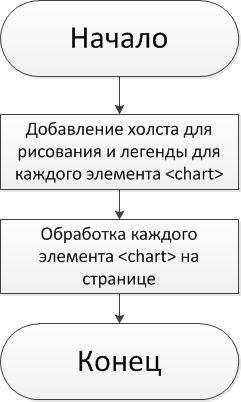
\includegraphics{start.png}}
\caption{Блок-схема функции запуска отрисовки графиков}
\label{ris:image}
\end{figure}
\subsection{Добавление\enspaceэлемента\enspaceв\enspaceлегенду}
\hspace{4ex}Данная функция предназначена для добавления названия элемента в легенду. Если имя пустое, то название запишется как 'serie'.
\begin{verbatim}
function legend_draw(legend, name, color, i) {
    var g = legend.append('g')
        .attr('transform', 
        'translate(0, ' + (i * 20 + 5 * i + 5) + ')')
    g.append('rect')
        .attr("width", 10)
        .attr("height", 10)
        .attr("fill", !color ? 'red' : color)
        .attr('x', 5)
        .attr('y', 5);
    g.append('text')
        .text(!name ? 'serie' : name)
        .attr('x', 20)
        .attr('y', 15);
}
\end{verbatim}
\begin{figure}[h]
\center{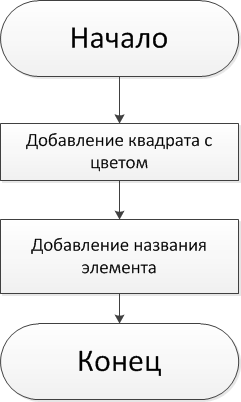
\includegraphics{legend_draw.png}}
\caption{Блок-схема функции добавления названия элемента в легенду}
\label{ris:image}
\end{figure}
\subsection{Обработка\enspaceэлемента\enspace<chart>\enspaceв\enspaceзависимости\enspaceот\enspaceтипа}
\hspace{4ex}Данная функция проверяет, какое значение аттрибута \textit{type} элемента <chart> присвоенно разработчиком для дальнейшего выбора условий отрисовки. Всего возможны варианты:
\begin{enumerate}
	\item \textit{undefined} (данное значение будет распозноваться библиотекой как значение "\textit{numeric}").
	\item \textit{numeric} (используется для отображения графиков). Также у данного типа есть свои виды отображения, которые могут сочетаться на одном графике:
	\begin{itemize}
		\item \textit{undefined} (данное значение будет распозноваться библиотекой как значение "\textit{point}").
		\item \textit{point} (отображает набор точек из данных из аттрибута \textit{data}).
		\item \textit{line} (отображает ломанную линию из данных из аттрибута \textit{data}).
		\item \textit{spline} (отображает плавную линию из данных из аттрибута \textit{data}).
	\end{itemize}	 
	\item \textit{pie} (используется для отображения круговых диаграмм).
	\item \textit{bar} (используется для отображения гистограмм).
	\item \textit{3d-pie} (используется для отображения объемных круговых диаграмм).
	\item \textit{3d-circle} (идинтичен \textit{3d-pie}, только с отверстием посередине).
	
\end{enumerate}
\begin{figure}[h]
\center{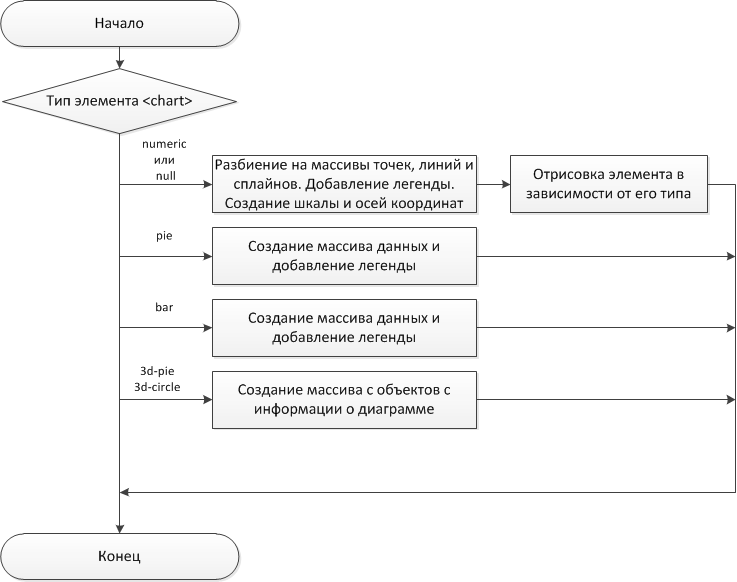
\includegraphics[scale=0.7]{series.png}}
\caption{Блок-схема функции обработки типа элемента <chart>}
\label{ris:image}
\end{figure}
\subsection{Получение\enspaceобласти\enspaceотображения\enspaceзначений\enspaceграфика}
\hspace{4ex}Функция предназначена для определения минимального и максимального значения для графика.
\begin{verbatim}
function getDomain(data, index) {
    var d = [];
    data.forEach(function(v) {
        v.forEach(function(v) {
            d.push(v[index])
        })
    });
    return [d.reduce(function(prev, next) {
            return Math.min(prev, next);
        }),
        d.reduce(function(prev, next) {
            return Math.max(prev, next);
        })
    ];
}
\end{verbatim}
\begin{figure}[h]
\center{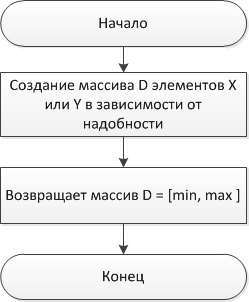
\includegraphics{getDomain.png}}
\caption{Блок-схема функции получения области отображения значений графика}
\label{ris:image}
\end{figure}
\subsection{Получение\enspaceмассива\enspaceзначений\enspaceдля\enspaceграфика}
\hspace{4ex}Главной задачей данной функции является выделение всех включений шаблона "[число число]" и преобразование полученных данных в массив.
\begin{verbatim}
function getPointData(seriesSet) {
    var data = [];
    seriesSet.forEach(function(val) {
        data.push(
            val.attr('data')
            .match(/\[ *(-|\+)?(\d+|\d+\.\d+) +?
(-|\+)?(\d+|\d+\.\d+) *\]/g)
            .map(function(val) {
                return JSON.parse(val.replace(/ +?/, ','));
            })
        )
    });
    return data;
}
\end{verbatim}
\begin{figure}[h]
\center{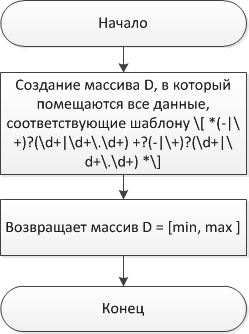
\includegraphics{getPointData.png}}
\caption{Блок-схема функции получения массива значений для графиков}
\label{ris:image}
\end{figure}
\subsection{Создание\enspaceшкалы\enspaceдля\enspaceграфика}
\hspace{4ex}При вызове данной функции происхоит поиск минимального и максимального значения графика, рисуются шкалы и возвращается функции, для шкал.
\newpage
\begin{figure}[h]
\center{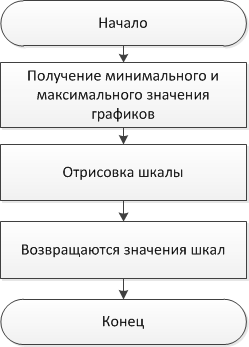
\includegraphics{createNumericScales.png}}
\caption{Блок-схема функции создания шкалы для графиков}
\label{ris:image}
\end{figure}
\subsection{Отрисовка\enspaceточек\enspaceна\enspaceграфике}
\hspace{4ex}Данная функция отрисовывает точки на графике с учетом данных, переданных функции и шкалы для определения положения точки на графике. Точки рисовались с помощью SVG элемента \textit{circle} с радиусом в 3 пикселя.
\hspace{4ex}Данная функция также предусматривает показ координат точки с помошью всплываюшей подсказки (tooltip).
\begin{verbatim}
d3.select(this).on("mouseenter", function() {
    element.select('.tip').attr('class', 'tip vis')
        .style('top', (scales.yScale(d[1])) + 'px')
        .style('left', scales.xScale(d[0]) + 'px');
    element.select('.tip').select('.s').text('Serie: point');
    element.select('.tip').select('.p')
        .text('X: ' + d[0] + ', Y:' + d[1]);
})
d3.select(this).on("mouseleave", function() {
    element.select('.tip').attr('class', 'tip');
})
\end{verbatim}
\newpage
\begin{figure}[h]
\center{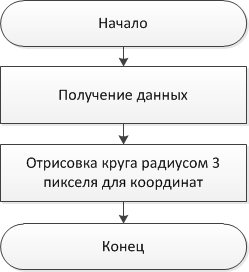
\includegraphics{point.png}}
\caption{Блок-схема функции отрисовки точек на графике}
\label{ris:image}
\end{figure}
\subsection{Отрисока\enspaceломанных\enspaceлиний\enspaceи\enspaceсплайнов\enspaceна\enspaceграфике}
\hspace{4ex}При вызове данной функции на графике появляются ломанные линии, узлы которых задаются разработчиком в html-документе и в последствии преобразовываются в массив координат.\\
\hspace{4ex}Данная функция способна преобразовать ломанные линии в плавные линии (сплайны). Для этого в параметры функции необходимо пятым параметром передать значение \textit{true}.
\begin{verbatim}
var line = d3.svg.line()
    .x(function(d) {
        return scales.xScale(d[0]);
    })
    .y(function(d) {
        return scales.yScale(d[1]);
    })
if (spline) {
    line.interpolate("basis");
}
element.select('svg').append('path')
    .attr('d', line(v))
    .attr('stroke', colors[i])
    .attr('stroke-width', 2)
    .attr('fill', 'none')
i++;
\end{verbatim}
\hspace{4ex}Также функция отрисовки линий, как и функция рендеринга точек, при наведении курсором мышки на линию появится всплывающая подсказка о текущих координатах точки графика.
\subsection{Отрисока\enspaceкруговой\enspaceдиаграммы}
\hspace{4ex}Отображение круговой диаграммы производится с помошью функции библиотеки D3.js. Для этого необходимо полученным данным из html-документа присвоить метку \textit{d3.layout.pie()}.\\
\begin{figure}[h]
\center{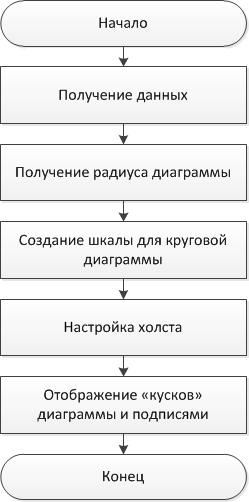
\includegraphics{pie.png}}
\caption{Блок-схема функции отображения круговой диаграммы}
\label{ris:image}
\end{figure}
\hspace{4ex}При наведение курсора мышки на диаграмму, остается подсвеченной только та её часть, внутри которой находится указатель.
\subsection{Создание\enspaceшкал\enspaceдля\enspaceгистограммы}
\hspace{4ex}При выполнении данной функции на текущем SVG-элементе появляется шкала, у которой по оси абсцис расположены цифры от 0 до максимального значения элементов гистограммы, а на оси ординат --- названия колонок.
\hspace{4ex}В итоге, функция возващает объект, у котороего есть два поля:
\begin{enumerate}
	\item Шкала X
	\item Шкала Y
\end{enumerate}
\begin{verbatim}
var yScale = d3.scale.linear()
    .range([height - margins.top,
        margins.bottom
    ])
    .domain(yDomain);

var xAxis = d3.svg.axis()
    .scale(xScale)
    .orient("bottom");

var yAxis = d3.svg.axis()
    .scale(yScale)
    .orient("left");
element.select('svg').append("g")
    .attr("class", "axis x")
    .attr("transform", "translate(0," + (height - margins.bottom) + ")")
    .call(xAxis);
element.select('svg').append("g")
    .attr("class", "axis y")
    .attr("transform", "translate(" + (margins.left) + ",0)")
    .call(yAxis);
return {x: xScale, y:yScale};
\end{verbatim}
\subsection{Отображение\enspaceгистограммы}
\hspace{4ex}Функция отображения предназначена для отрисовки SVG-элементов \textit{rect} расположенных верникально. Ширина столбцов определяется автоматически с помощью функции \textit{.rangeBand()} у шкалы X.
\newpage
\begin{figure}[h]
\center{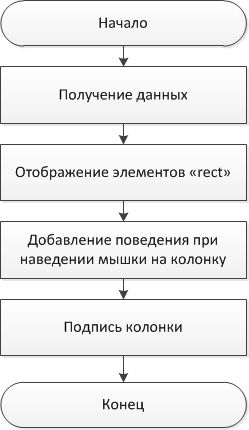
\includegraphics{bar.png}}
\caption{Блок-схема функции отображения гистограммы}
\label{ris:image}
\end{figure}
\hspace{4ex}При наверении мышкой на столбец, все элементы, кроме выбранного пракически исчезают, что наглядно показывает, какой элемент выбран на данный момент.
\subsection{3D\enspaceэлементы}
\hspace{4ex}Элементы выполненные в 3D-формате (объемная круговая диаграмма и объемная кольцевая диаграмма) выполнены в отдельном файле 3D.js, в котором присутствует анонимная самовызывающая функция, главным элементом которой является объект Donut3D. Отрисовка выполняется поочередным отображением сперва внутренней, потом верхней, а затем внешней границы сектора объемной диагаммы.
\newpage
\begin{figure}[h]
\center{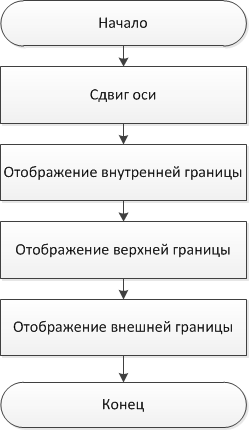
\includegraphics{3D.png}}
\caption{Блок-схема функции отображения 3D-элементов}
\label{ris:image}
\end{figure}
\chapter{Тестирование\enspaceпрограммного\enspaceсредства}
\hspace{4ex}Тестирование данного ПС было сделано с использованием библиотек:
\begin{itemize}
	\item \textit{mocha.js} (служит средой для запуска тестов)
	\item \textit{chai.js} (служит для облегчения понимания написанных тестов, более читабельного кода)
	\item \textit{sinon.js} (предоставляет элемент spy() для тестирования функций)
	\item \textit{sinon-chai.js} (служит для служит для облегчения понимания тестов, написанных с использованием элементов spy())
\end{itemize}
\hspace{4ex}Код unit-тестов находится в Приложении-Б.
\begin{figure}[h]
\center{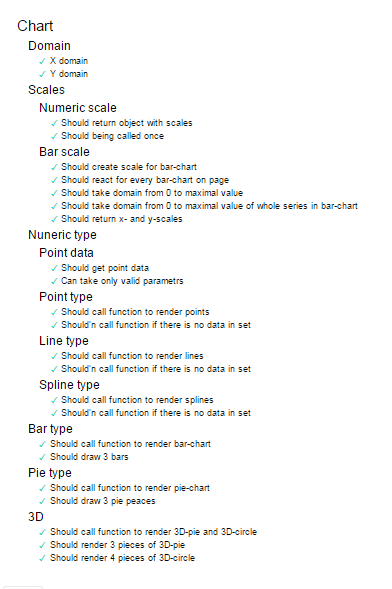
\includegraphics[scale=0.86]{tests.png}}
\caption{Результаты тестов}
\label{ris:image}
\end{figure}
\chapter{Руководство\enspaceпользователя}
\section{Установка}
\subsection{Установка\enspaceчерез\enspace npm}
\hspace{4ex}Для установки данным способом необходимо, чтобы на компьютере был установлен \textbf{node.js} и \textbf{npm}.
\hspace{4ex}Необходимо зайти в папку, куда должен быть установлен пакет, и ввести комманду:
\begin{verbatim}
    npm install chart-js-d3 --save
\end{verbatim}
\begin{figure}[h]
\center{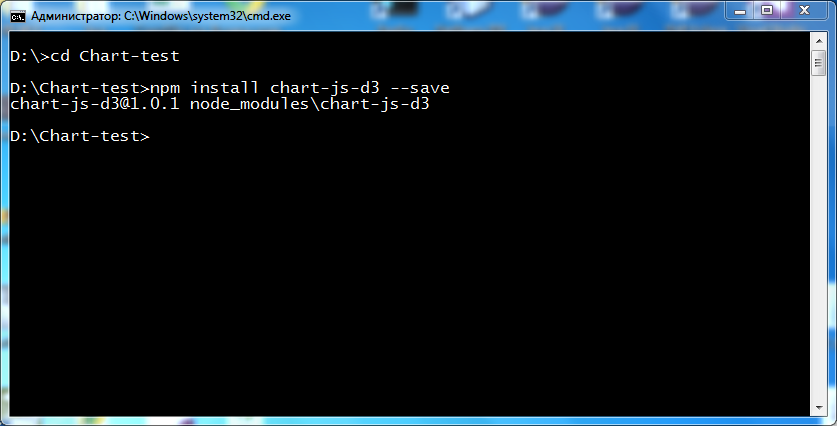
\includegraphics[scale=0.75]{npm.png}}
\caption{Установка через npm}
\label{ris:image}
\end{figure}
\hspace{4ex}Для работы библиотеки, обязательно нужно подключить следующий пречешь файлов в html-документ в такойже последовательности:
\begin{verbatim}
    <script src="node_modules/chart-js-d3/lib/d3.min.js"></script>
    <script src="node_modules/chart-js-d3/js/3d.js"></script>
    <script src="node_modules/chart-js-d3/js/chart.js"></script>
\end{verbatim}
\hspace{4ex}Далее на html-страницу желательно подключить стандартные стили разработчика:
\begin{verbatim}
    <link rel="stylesheet" type="text/css" 
    href="node_modules/chart-js-d3/css/style.css">
\end{verbatim} 
\newpage
\begin{figure}[h]
\center{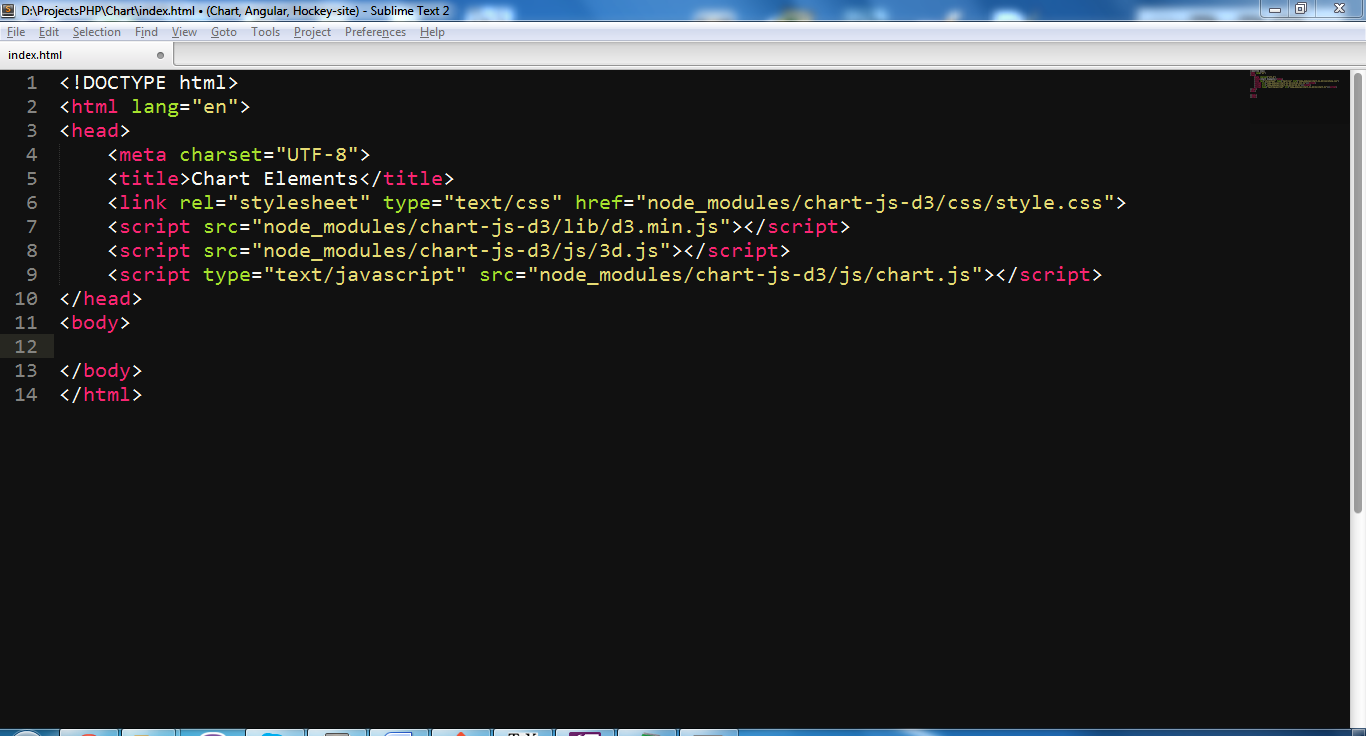
\includegraphics[scale=0.45]{screen_npm.png}}
\caption{Желательный первоначальный html-файл}
\label{ris:image}
\end{figure}
\subsection{Скачать\enspaceдемо-проект\enspaceс\enspace GitHub}
\hspace{4ex}Есть возможность скачать или склонировать демо-проект с GitHub по адресу: \\
\hspace{4ex}\textbf{\href{https://github.com/AlekseyKasteuk/Chart-js-d3}{https://github.com/AlekseyKasteuk/Chart-js-d3}}
\newpage
\begin{figure}[h]
\center{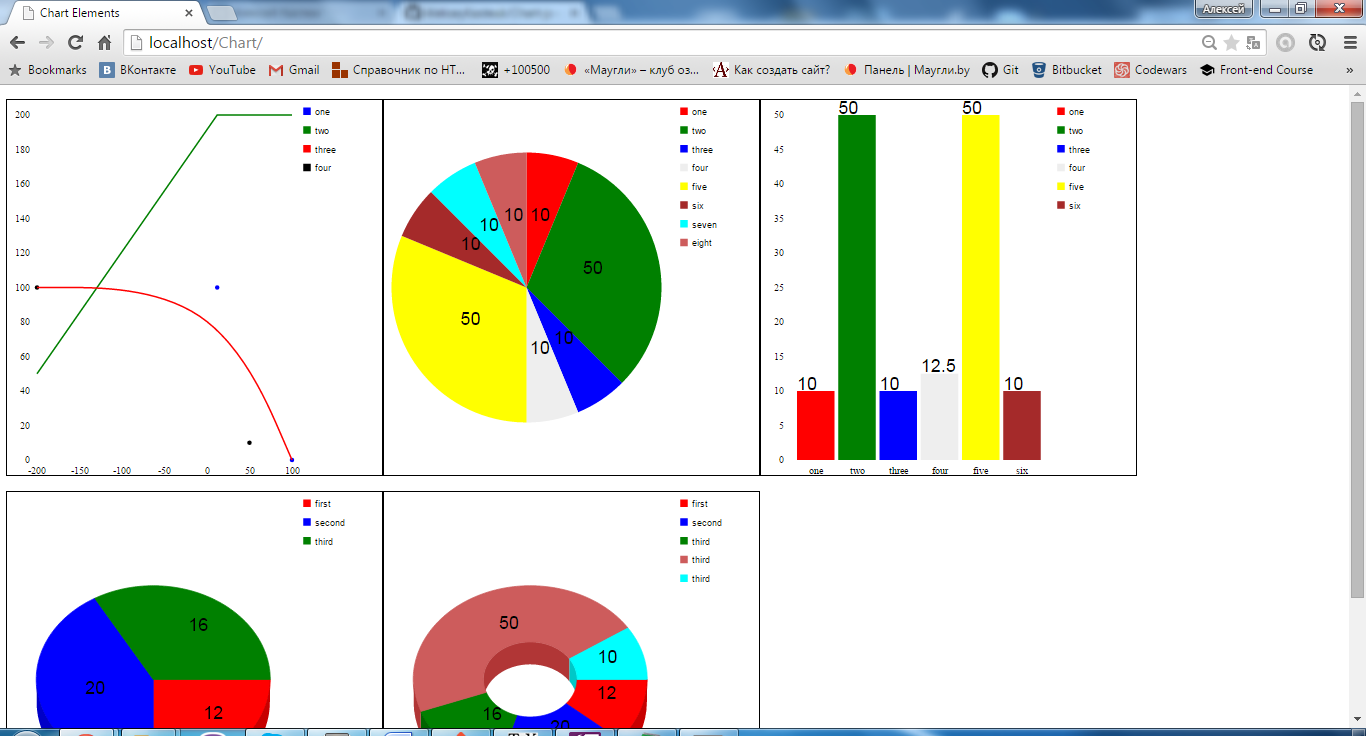
\includegraphics[scale=0.45]{demo.png}}
\caption{Демо-файл}
\label{ris:image}
\end{figure}
\section{Использование}
\hspace{4ex}Для отображения графика на странице необходимо записать тег <chart></chart>, внутри которого нужно вставить тег <section></section> с определенным набором параметров, которые возможно найти в главе \hyperref[2.3.3]{2.3.3}
\newpage
\begin{figure}[h]
\center{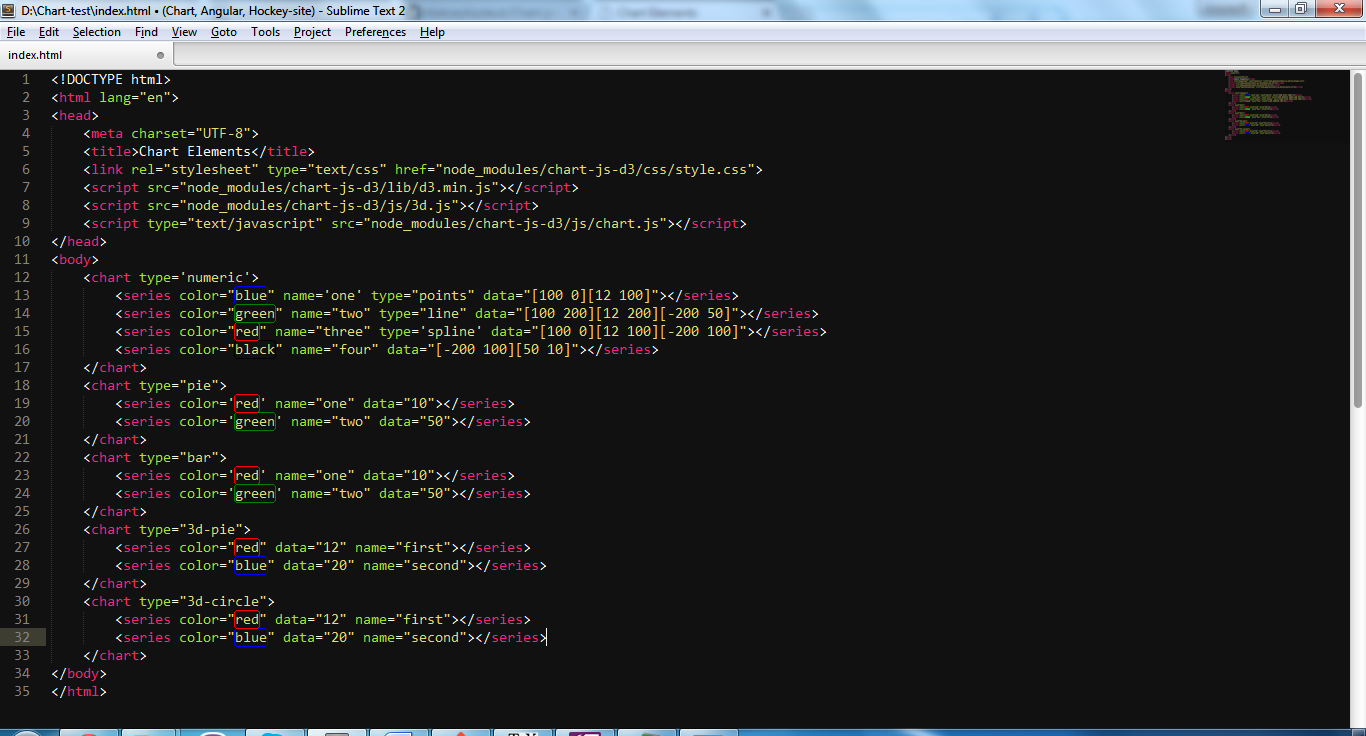
\includegraphics[scale=0.45]{useing.png}}
\caption{Пример кода использования}
\label{ris:image}
\end{figure}
\begin{figure}[h]
\center{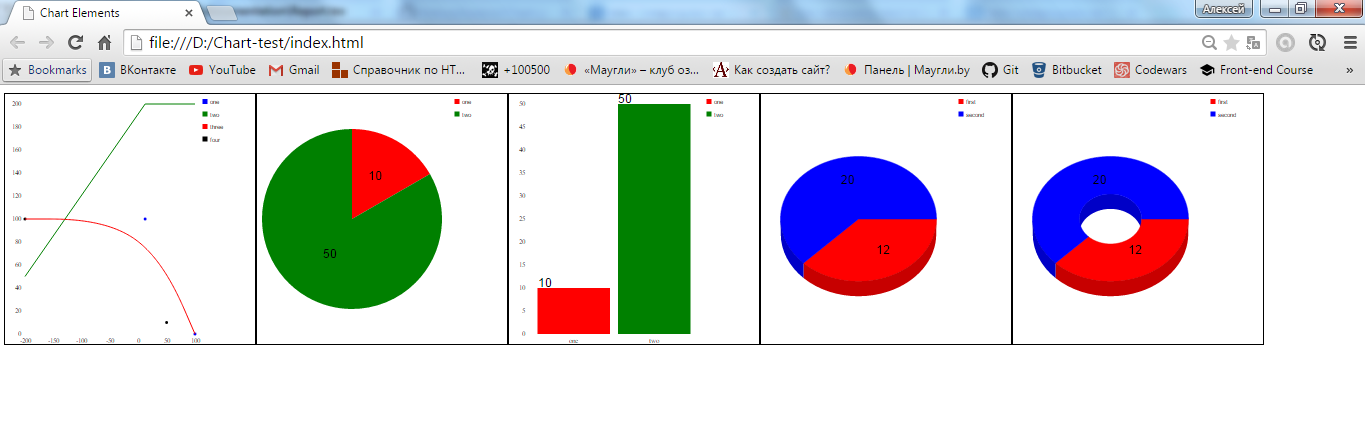
\includegraphics[scale=0.45]{useing_.png}}
\caption{Результат}
\label{ris:image}
\end{figure}
\newpage
\addcontentsline{toc}{chapter}{Заключение}
\chapter*{Заключение}
\hspace{4ex}В результате выполнения курсового проекта была разработана библиотека, предназначенная для отображения графиков и диаграмм на веб-странице.\\
\hspace{4ex}Проект был выполнен на языке Javascript с использованием библиотеки D3.js. Тестирование программы было выполнено с использованием библиотек mocha.js, chai.js, sinon.js, sinon-chai.js.\\
\hspace{4ex}В дальнейшем библиотека может быть расширена новыми видами графиков, такими как:
\begin{itemize}
	\item Биржевой график
	\item Поверхностный график
	\item График с областями
\end{itemize}
\newpage
\addcontentsline{toc}{chapter}{Список использованной литературы}
\chapter*{Список\enspaceиспользованной\enspaceлитературы}
\begin{thebibliography}{9}
\bibitem{http://d3js.org} Data-Driven Documents d3js.org
\bibitem{} David Flanagan JavaScript: Подробное руководство (Definitive Guide)
\bibitem{} Хоган Б. HTML5 и CSS3. Веб-разработка по стандартам нового поколения. 2-е изд.
\end{thebibliography}
\newpage
\addcontentsline{toc}{chapter}{Приложение A}
\chapter*{\centerПриложение\enspaceА\\(обязательное)\\Исходный код программы\endcenter}
\section*{chart.js}
\begin{lstlisting}
window.onload = start;
window.onresize = function() {
  d3.selectAll("chart").select("svg").remove();
  d3.selectAll("chart").select(".tip").remove();
  start();
}

function start() {
  d3.selectAll("chart")
    .append('svg')
    .append('g')
    .attr('class', 'legend');
  d3.selectAll('chart').append('div').attr('class', 'tip')
    .html("<div class='s'></div><div class='p'></div>")
  d3.selectAll('chart')[0].forEach(function(val) {
    series(d3.select(val));
  });
};

function legend_draw(legend, name, color, i) {
  var g = legend.append('g')
    .attr('transform', 'translate(0, ' + (i * 20 + 5 * i + 5) + ')')
  g.append('rect')
    .attr("width", 10)
    .attr("height", 10)
    .attr("fill", !color ? 'red' : color)
    .attr('x', 5)
    .attr('y', 5);
  g.append('text')
    .text(!name ? 'serie' : name)
    .attr('x', 20)
    .attr('y', 15);
}

function series(element) {
  var width = element.style("width").slice(0, -2);
  var height = element.style("height").slice(0, -2);
  switch (element.attr('type')) {
    case null:
    case 'numeric':
      var pointSet = [];
      var lineSet = [];
      var splineSet = [];
      var pointsColor = [];
      var linesColor = [];
      var splineColor = [];
      var wholePoints;
      var scales;
      var i = 0;
      var legend = element
        .select('.legend')
        .attr('transform', 'translate(' + (width - 110) + ', 0)')
      element.selectAll('series')[0].forEach(function(val) {
        var type = d3.select(val).attr('type');
        var color = d3.select(val).attr('color');
        var name = d3.select(val).attr('name');
        if (type == 'points' || type == undefined) {
          if (d3.select(val).attr('data')) {
            pointSet.push(d3.select(val));
            pointsColor.push(!color ? 'red' : color);
          }
        }
        if (type == 'line') {
          if (d3.select(val).attr('data')) {
            lineSet.push(d3.select(val));
            linesColor.push(!color ? 'red' : color);
          }
        }
        if (type == 'spline') {
          if (d3.select(val).attr('data')) {
            splineSet.push(d3.select(val));
            splineColor.push(!color ? 'red' : color);
          }
        }
        legend_draw(legend, name, color, i)
        i++;
      });
      wholePoints = pointSet.concat(lineSet).concat(splineSet);
      if (wholePoints.length) {
        scales = createNumericScales(element, wholePoints);
      } else {
        return;
      }
      if (pointSet.length) {
        points(element, pointSet, scales, pointsColor);
      }
      if (lineSet.length) {
        lines(element, lineSet, scales, linesColor)
      }
      if (splineSet.length) {
        lines(element, splineSet, scales, splineColor, true)
      }
      break;
    case 'pie':
      var pieData = [];
      var pieColors = [];
      var legend = element
        .select('.legend')
        .attr('transform', 'translate(' + (width - 110) + ', 0)');
      var i = 0;
      element.selectAll('series')[0].forEach(function(val) {
        var color = d3.select(val).attr('color');
        var name = d3.select(val).attr('name');
        var data = d3.select(val).attr('data');
        try {
          data = !data ? 0 :
          data.match(/^( *)\d+(\.\d+)?( *)$/g)[0];
        }
        catch(e) {
          data = 0;
        }
        if(!color) { color = 'red' }
        if(!name) { name = 'pie pice' }
        pieColors.push(color);
        pieData.push({data: data, name: name});
        legend_draw(legend, name, color, i)
        i++;
      });
      pie(element, pieData, pieColors);
      break;
    case 'bar':
      var bars = [];
      var wholeData = [];
      var wholeNames = [];
      var i = 0, count = 1;
      var legend = element
        .select('.legend')
        .attr('transform', 'translate(' + (width - 110) + ', 0)');
      element.selectAll('series')[0].forEach(function(val) {
        var color = d3.select(val).attr('color');
        var name = d3.select(val).attr('name');
        var data = d3.select(val).attr('data');
        try {
          data = !data ? 0 :
          data.match(/^( *)\d+(\.\d+)?( *)$/g)[0];
        }
        catch(e) {
          data = 0;
        }
        if(!data) { data = [0] }
        if(!color) { color = 'red' }
        if(!name) { name = 'bar_' + i }
        wholeData = wholeData.concat(data);
        while(wholeNames.indexOf(name) != -1) { name += "_" + i }
        wholeNames.push(name);
        bars.push({color: color, name: name, data: data});
        legend_draw(legend, name, color, i)
        i++;
      });
      wholeData = wholeData.map(function(v) { return v - 0 });
      bar(element,
      createBarsScale(element, wholeData, wholeNames,
        [0, wholeData.reduce(function(prev, next){
          return Math.max(prev, next)
        })]),
      bars);
      break;
    case '3d-circle':
    case '3d-pie': 
      var data3d = [];
      var colors = [];
      var legend = element
        .select('.legend')
        .attr('transform', 'translate(' + (width - 110) + ', 0)');
      var i = 0;
      element.selectAll('series')[0].forEach(function(val) {
        var color = d3.select(val).attr('color');
        var name = d3.select(val).attr('name');
        var data = d3.select(val).attr('data');
        try {
          data = !data ? 0 :
          data.match(/^( *)\d+(\.\d+)?( *)$/g)[0];
        }
        catch(e) {
          data = 0;
        }
        data = parseInt(data);
        if(!color) { color = 'red' }
        if(!name) { name = 'pie pice' }
        if(!data) { data = 0 }
        colors.push(color);
        data3d.push({value: data, label: name, color: color});
        legend_draw(legend, name, color, i);
        i++;
      });
      var r = width - 110 < height ? (width - 110) / 2 : height / 2;
      var ir = element.attr('type') == "3d-pie" ? 0 : 0.4;
      Donut3D.draw(element, data3d, (width - 110) / 2, height / 2, (width - 110) / 2.5, height / 4, 30, ir);
      break;
    default:
      break;
  }
}

function getDomain(data, index) {
  var d = [];
  data.forEach(function(v) {
    v.forEach(function(v) {
      d.push(v[index])
    })
  });
  return [d.reduce(function(prev, next) {
      return Math.min(prev, next);
    }),
    d.reduce(function(prev, next) {
      return Math.max(prev, next);
    })
  ];
}

function getPointData(seriesSet) {
  var data = [];
  seriesSet.forEach(function(val) {
    data.push(
      val.attr('data')
      .match(/\[ *(-|\+)?(\d+|\d+\.\d+) +?(-|\+)?(\d+|\d+\.\d+) *\]/g)
      .map(function(val) {
        return JSON.parse(val.replace(/ +?/, ','));
      })
    )
  });
  return data;
}

function createNumericScales(element, seriesSet) {
  var data = getPointData(seriesSet);
  var width = element.style("width").slice(0, -2);
  var height = element.style("height").slice(0, -2);
  var margins = {
    left: 40,
    right: 120,
    top: 20,
    bottom: 20
  }
  var xDomain = getDomain(data, 0);
  var yDomain = getDomain(data, 1);
  var xScale = d3.scale.linear()
    .range([margins.left,
      width - margins.right
    ])
    .domain(xDomain);
  var yScale = d3.scale.linear()
    .range([height - margins.top,
      margins.bottom
    ])
    .domain(yDomain);
  var xAxis = d3.svg.axis().scale(xScale);
  var yAxis = d3.svg.axis().scale(yScale)
    .orient('left');
  element.select('svg').append("g")
    .attr("class", "axis x")
    .attr("transform", "translate(0," + (height - margins.bottom) + ")")
    .call(xAxis);
  element.select('svg').append("g")
    .attr("class", "axis y")
    .attr("transform", "translate(" + (margins.left) + ",0)")
    .call(yAxis);
  return {
    xScale: xScale,
    yScale: yScale
  };
}

function points(element, set, scales, colors) {
  var data = getPointData(set);
  var i = 0;
  data.forEach(function(v) {
    element.select('svg').append('g')
      .selectAll('circle').data(v)
      .enter()
      .append('circle')
      .attr('cx', function(d) {
        d3.select(this).on("mouseenter", function() {
          element.select('.tip').attr('class', 'tip vis')
            .style('top', (scales.yScale(d[1])) + 'px')
            .style('left', scales.xScale(d[0]) + 'px');
          element.select('.tip').select('.s').text('Serie: point');
          element.select('.tip').select('.p').text('X: ' + d[0] + ', Y:' + d[1]);
        })
        d3.select(this).on("mouseleave", function() {
          element.select('.tip').attr('class', 'tip');
        })
        return scales.xScale(d[0]);
      })
      .attr('cy', function(d) {
        return scales.yScale(d[1]);
      })
      .attr('r', 3)
      .attr('fill', colors[i])
    i++;
  });
}

function lines(element, set, scales, colors, spline) {
  var data = getPointData(set);
  var i = 0;
  data.forEach(function(v) {
    var line = d3.svg.line()
      .x(function(d) {
        return scales.xScale(d[0]);
      })
      .y(function(d) {
        return scales.yScale(d[1]);
      })
    if (spline) {
      line.interpolate("basis");
    }
    element.select('svg').append('path')
      .attr('d', line(v))
      .attr('stroke', colors[i])
      .attr('stroke-width', 2)
      .attr('fill', 'none')
      .on("mouseenter", function() {
        var d = d3.mouse(this);
        element.select('.tip').attr('class', 'tip vis')
          .style('top', d[1] + 'px')
             .style('left', d[0] + 'px');
        element.select('.tip').select('.s').text('Serie: line');
        element.select('.tip')
          .select('.p')
          .text('X: ' + (Math.round(scales.xScale.invert(d[0]) * 1000) / 1000) +
            ', Y:' + (Math.round(scales.yScale.invert(d[1]) * 1000) / 1000));
      })
      .on("mouseleave", function() {
        element.select('.tip').attr('class', 'tip');
      })
    i++;
  });
}

function pie(element, data, colors) {
  var width = element.style("width").slice(0, -2) - 120;
  var height = element.style("height").slice(0, -2);
  var radius = Math.min(width, height) / 2;
  var color = d3.scale.ordinal().range(colors);
  var arc = d3.svg.arc()
    .outerRadius(radius - 10)
    .innerRadius(0);
  var pie = d3.layout.pie()
    .sort(null)
    .value(function(d) { return d.data; })
  var svg = element.select('svg')
    .data([data])
    .append('g')
    .attr("transform", "translate(" + width / 2 + "," + height / 2 + ")");
  var arcs = svg.selectAll("g.slice")
    .data(pie)
    .enter()              
    .append("svg:g")        
      .attr("class", "slice")
      .on('mouseenter', function() {
        d3.select(this.parentNode).selectAll('.slice').attr('opacity', '0.1');
        d3.select(this).attr('opacity', 1);
      })
      .on('mouseleave', function() {
        d3.select(this.parentNode).selectAll('.slice').attr('opacity', null);
      })
    arcs.append("svg:path")
      .attr("fill", function(d, i) { return color(i); } ) 
      .attr("d", arc);
    arcs.append("svg:text")                   
      .attr("transform", function(d) {
      d.innerRadius = 0;
      d.outerRadius = radius;
      return "translate(" + arc.centroid(d) + ")";    
    })
    .attr("text-anchor", "middle")              
    .text(function(d, i) { return data[i].data; });  
}

function createBarsScale(element, data, names, yDomain) {
  var width = element.style("width").slice(0, -2);
  var height = element.style("height").slice(0, -2);
  var margins = {
    left: 40,
    right: 120,
    top: 20,
    bottom: 20
  }
  var xScale = d3.scale.ordinal()
    .rangeRoundBands([margins.left,
      width - margins.right
    ], .1)
    .domain(names.map(function(d) { return d; }));
  var yScale = d3.scale.linear()
    .range([height - margins.top,
      margins.bottom
    ])
    .domain(yDomain);

  var xAxis = d3.svg.axis()
    .scale(xScale)
    .orient("bottom");

  var yAxis = d3.svg.axis()
    .scale(yScale)
    .orient("left");
  element.select('svg').append("g")
    .attr("class", "axis x")
    .attr("transform", "translate(0," + (height - margins.bottom) + ")")
    .call(xAxis);
  element.select('svg').append("g")
    .attr("class", "axis y")
    .attr("transform", "translate(" + (margins.left) + ",0)")
    .call(yAxis);
  return {x: xScale, y:yScale};
}

function bar(element, scales, data) {
  var height = element.style("height").slice(0, -2);
  var svg = element.select('svg').append("g")
    .attr("class", "bars")
  svg.selectAll(".bar")
    .data(data)
    .enter().append("rect")
    .attr("class", "bar")
    .style("fill", function(d) {return d.color; })
    .attr("x", function(d) { return scales.x(d.name); })
    .attr("width", function() {  return scales.x.rangeBand() })
    .attr("y", function(d) { return scales.y(d.data); })
    .attr("height", function(d) { return height - scales.y(d.data) - 20; })
    .on('mouseenter', function() {
       d3.select(this.parentNode).selectAll('rect').attr('opacity', '0.1');
    d3.select(this).attr('opacity', 1);
     })
     .on('mouseleave', function() {
    d3.select(this.parentNode).selectAll('rect').attr('opacity', null);
     })
  svg.selectAll("text")
    .data(data)
    .enter().append("text")
    .attr("x", function(d) { return scales.x(d.name); })
    .attr("y", function(d) { return scales.y(d.data) - 2; })
    .attr("font-family", "sans-serif")
    .attr("font-size", '14')
    .text(function(d) { return d.data })
}
\end{lstlisting}
\section*{3d.js}
\begin{lstlisting}
(function(){
  var Donut3D={};
  
  function pieTop(d, rx, ry, ir ){
    if(d.endAngle - d.startAngle == 0 ) return "M 0 0";
    var sx = rx * Math.cos(d.startAngle),
      sy = ry * Math.sin(d.startAngle),
      ex = rx * Math.cos(d.endAngle),
      ey = ry * Math.sin(d.endAngle);
      
    var ret = [];
    ret.push("M", sx, sy, "A", rx, ry, "0",
      (d.endAngle - d.startAngle > Math.PI? 1: 0), "1", ex, ey, "L", ir * ex, ir * ey);
    ret.push("A", ir * rx, ir * ry, "0", (d.endAngle - d.startAngle > Math.PI ? 1 : 0), "0", ir * sx, ir * sy, "z");
    return ret.join(" ");
  }

  function pieOuter(d, rx, ry, h){
    var startAngle = (d.startAngle > Math.PI ? Math.PI : d.startAngle);
    var endAngle = (d.endAngle > Math.PI ? Math.PI : d.endAngle);
    
    var sx = rx * Math.cos(startAngle),
      sy = ry * Math.sin(startAngle),
      ex = rx * Math.cos(endAngle),
      ey = ry * Math.sin(endAngle);
      
      var ret =[];
      ret.push("M", sx, h + sy, "A", rx, ry, "0 0 1", ex, h + ey, "L", ex, ey, "A", rx, ry, "0 0 0", sx, sy, "z");
      return ret.join(" ");
  }

  function pieInner(d, rx, ry, h, ir ){
    var startAngle = (d.startAngle < Math.PI ? Math.PI : d.startAngle);
    var endAngle = (d.endAngle < Math.PI ? Math.PI : d.endAngle);
    
    var sx = ir * rx * Math.cos(startAngle),
      sy = ir * ry * Math.sin(startAngle),
      ex = ir * rx * Math.cos(endAngle),
      ey = ir * ry * Math.sin(endAngle);

      var ret = [];
      ret.push("M", sx, sy, "A", ir * rx, ir * ry, "0 0 1", ex, ey, "L", ex, h + ey, "A", ir * rx, ir * ry, "0 0 0", sx, h + sy, "z");
      return ret.join(" ");
  }
  
  Donut3D.draw=function(element, data, x, y, rx, ry, h, ir){
  
    var _data = d3.layout.pie().sort(null).value(function(d) { return d.value; })(data);
    
    var slices = element.select("svg").append("g").attr("transform", "translate(" + x + "," + y + ")")
      .attr("class", "slices");

    slices.selectAll(".innerSlice").data(_data).enter().append("path").attr("class", "innerSlice")
      .style("fill", function(d) { return d3.hsl(d.data.color).darker(0.7); })
      .attr("d",function(d){ return pieInner(d, rx+0.5,ry+0.5, h, ir);})
      .each(function(d){this._current=d;});
    
    slices.selectAll(".topSlice").data(_data).enter().append("path").attr("class", "topSlice")
      .style("fill", function(d) { return d.data.color; })
      .style("stroke", function(d) { return d.data.color; })
      .attr("d",function(d){ return pieTop(d, rx, ry, ir);})
      .each(function(d){this._current=d;});
    
    slices.selectAll(".outerSlice").data(_data).enter().append("path").attr("class", "outerSlice")
      .style("fill", function(d) { return d3.hsl(d.data.color).darker(0.7); })
      .attr("d",function(d){ return pieOuter(d, rx - .5,ry - .5, h);})
      .each(function(d){this._current = d;});

    slices.selectAll(".value").data(_data).enter().append("text").attr("class", "value")
      .attr("x",function(d){ return 0.6 * rx * Math.cos(0.5 * (d.startAngle + d.endAngle));})
      .attr("y",function(d){ return 0.6 * ry * Math.sin(0.5 * (d.startAngle + d.endAngle));})
      .text(function(d){ return d.value});        
  }
  
  this.Donut3D = Donut3D;
})();
\end{lstlisting}
\section*{style.css}
\begin{lstlisting}
chart {
  width: 500px;
  height: 500px;
  display: block;
  position: relative;
  margin: 10px 0;
  min-width: 300px !important;
  min-height: 300px !important;
  border: 1px solid black;
}

svg {
  height: 100%;
  width: 100%;
  margin: 0;
  padding: 0;
  overflow: visible;
}

.legend {
  height: 100%;
  width: 20%;
  margin: 0;
  padding: 0;
}

.axis path {
  fill: none;
  stroke: #777;
  shape-rendering: crispEdges;
}
.axis  text {
  font-family: Lato;
  font-size: 13px;
}

.x text {
  width: 10px;
  white-space: normal;
}

#info {
  fill: #aaa;
  color: red;
  margin: 0 auto;
  font-size: 16px;
}

.serie {
  padding: 5px;
  margin-bottom: 3px;
}

.serie_color {
  display: inline-block;
}

.serie_color~div {
  display: inline-block;
  margin-left: 5px;

}

.tip {
  width: 150px;
  height: 50px;
  background-color: black;
  position: absolute;
  visibility: hidden;
  color: white;
  padding: 5px;
  text-align: center;
  top: 0;
  margin: -75px -80px;
}

.tip::after {
  content: '';
  top: 60px;
  left: 75px;
  position: absolute;
  visibility: inherit;
    border-left: 5px solid transparent;
    border-right: 5px solid transparent;
    border-top: 10px solid black;
}

.vis {
  visibility: visible;
}

g text {
  font-size: 1.5em;
    font-family: Arial;
    cursor: default;
}

.legend text {
  font-size: 12px
}
\end{lstlisting}
\section*{chart.spec.js}
\begin{lstlisting}
describe('Chart', function () {
  describe('Domain', function() {
    it('X domain', function() {
      expect(getDomain([[[100, 300], [12, 100]],[[10, -1], [-100, 2]]], 0)).
        to.be.deep.equal([-100, 100]);
      expect(getDomain([[[3,1]], [[2,1], [3,1]]], 0)).not.
        to.be.deep.equal([2, 4]);
      expect(getDomain([[[0, 0]]], 0)).
        to.be.deep.equal([0, 0]);
    })
    it('Y domain', function() {
      expect(getDomain([[[100, 300], [12, 100]],[[10, -1], [-100, 2]]], 1)).
        to.be.deep.equal([-1, 300]);
      expect(getDomain([[[0, 0]]], 1)).
        to.be.deep.equal([0, 0]);
    })
  })
  describe('Scales', function () {
    describe('Numeric scale', function () {
      beforeEach(function() {
        var body =d3.select("body")
          .append("chart");
        body.append("series")
          .attr("type", "line")
          .attr("data", "[50 0]");
        body.append("series")
          .attr("type", "points")
          .attr("data", "[100 0][12 100]");
      })
      afterEach(function() {
        d3.selectAll("chart").remove();
      })
      it('Should return object with scales', function () {
        var pointsSpy = sinon.spy();
          lineSpy = sinon.spy();
        points = pointsSpy;
        lines = lineSpy;
        start();
        expect(pointsSpy).to.have.been.calledOnce;
        expect(lineSpy).to.have.been.calledOnce;
        expect(pointsSpy.args[0][2]).to.be.deep.equal(lineSpy.args[0][2]);
        expect(typeof pointsSpy.args[0][2].xScale).to.be.deep.equal('function');
        expect(typeof pointsSpy.args[0][2].yScale).to.be.deep.equal('function');
      })
      it('Should being called once', function () {
        var createNumericSpy = sinon.spy(),
          pointsSpy = sinon.spy();
          lineSpy = sinon.spy();
        createNumericScales = createNumericSpy;
        points = pointsSpy;
        lines = lineSpy;
        start();
        expect(createNumericSpy).to.have.been.calledOnce;
      })
    })
    describe('Bar scale', function () {
      var firstBarReleaze = bar,
        firstCreateBarScale = createBarsScale;
      afterEach(function() {
        d3.selectAll("chart").remove();
        bar = firstBarReleaze;
        createBarsScale = firstCreateBarScale;
      })
      it('Should create scale for bar-chart', function () {
        var spy = sinon.spy(),
          spyBar = sinon.spy();
        bar = spyBar;
        d3.select("body").append("chart").attr("type", "bar").append("series");
        createBarsScale = spy;
        start();
        expect(spy).to.have.been.calledOnce;
      })
      it('Should react for every bar-chart on page', function () {
        var spy = sinon.spy(),
          spyBar = sinon.spy();
        bar = spyBar;
        d3.select("body").append("chart").attr("type", "bar").append("series");
        d3.select("body").append("chart").attr("type", "bar").append("series");
        createBarsScale = spy;
        start();
        expect(spy).to.have.been.calledTwice;
      })
      it('Should take domain from 0 to maximal value', function () {
        var spy = sinon.spy(),
          spyBar = sinon.spy();
        bar = spyBar;
        d3.select("body").append("chart").attr("type", "bar").append("series")
          .attr("data", "10")
        d3.select("body").append("chart").attr("type", "bar").append("series");
        createBarsScale = spy;
        start();
        expect(spy.args[0][3]).to.be.deep.equal([0, 10]);
        expect(spy.args[1][3]).to.be.deep.equal([0, 0]);
      })
      it('Should take domain from 0 to maximal value of whole series in bar-chart', function () {
        var spy = sinon.spy(),
          spyBar = sinon.spy();
        bar = spyBar;
        var chart = d3.select("body").append("chart").attr("type", "bar");
        chart.append("series").attr("data", "10");
        chart.append("series").attr("data", "100");
        createBarsScale = spy;
        start();
        expect(spy.args[0][3]).to.be.deep.equal([0, 100]);
      })
      it('Should return x- and y-scales', function () {
        var spyBar = sinon.spy();
        bar = spyBar;
        var chart = d3.select("body").append("chart").attr("type", "bar");
        chart.append("series").attr("data", "10").attr("name", "test");
        start();
        expect(spyBar.args[0][1].y(0)).to.be.equal(480);
        expect(spyBar.args[0][1].y(10)).to.be.equal(20);
      })
    })
  })
  describe('Nuneric type', function () {
    describe('Point data', function () {
      beforeEach(function() {
        d3.select('body')
          .append('chart')
          .append('series')
          .attr('data', '[100 300][12 100]');
      })
      afterEach(function() {
        d3.select('chart')
          .remove();
      })
      it('Should get point data', function() {
        expect(getPointData([d3.select('series')]))
        .to.be.deep.equal
        ([[[100, 300], [12, 100]]]);
      })
      it('Can take only valid parametrs', function () {
        d3.select("series").attr("data", "asd[12 0]1[1 2]");
        expect(getPointData([d3.select('series')]))
        .to.be.deep.equal
        ([[[12, 0], [1, 2]]]);
      })
    })
    describe('Point type', function () {
      beforeEach(function() {
        var body =d3.select("body")
          .append("chart");
        body.append("series")
          .attr("data", "[100 0][12 100]");
        body.append("series")
          .attr("type", "points")
          .attr("color", "green")
          .attr("data", "[100 0][12 100]");
      })
      afterEach(function() {
        d3.select("chart").remove();
      })
      it('Should call function to render points', function () {
        var spy = sinon.spy();
        points = spy;
        start();
        expect(spy).to.have.been.calledOnce;
        expect(getPointData(spy.args[0][1])).to.be.deep.equal([[[100, 0],[12, 100]], [[100, 0], [12, 100]]]);
        expect(spy.args[0][3]).to.be.deep.equal(["red", "green"]);
      })
      it("Should'n call function if there is no data in set", function () {
        d3.select("chart").remove();
        var body =d3.select("body")
          .append("chart")
          .append("series")
          .attr("data", "");
        var spy = sinon.spy();
        points = spy;
        start();
        expect(spy).not.to.have.been.called;
      })
    })
    describe('Line type', function () {
      beforeEach(function() {
        var body =d3.select("body")
          .append("chart");
        body.append("series")
          .attr("type", "line")
          .attr("data", "[100 0][12 100]");
      })
      afterEach(function() {
        d3.select("chart").remove();
      })
      it('Should call function to render lines', function () {
        var spyPoints = sinon.spy(),
          spyLines = sinon.spy()
        points = spyPoints;
        lines = spyLines;
        start();
        expect(spyPoints).not.to.have.been.called;
        expect(spyLines).to.have.been.calledOnce;
        expect(getPointData(spyLines.args[0][1])).to.be.deep.equal([[[100, 0],[12, 100]]]);
        expect(!!spyLines.args[0][4]).to.be.equal(false);
      })
      it("Should'n call function if there is no data in set", function () {
        d3.select("chart").remove();
        var body =d3.select("body")
          .append("chart")
          .append("series")
          .attr("type", "line")
          .attr("data", "");
        var spy = sinon.spy();
        lines = spy;
        start();
        expect(spy).not.to.have.been.called;
      })
    })
    describe('Spline type', function () {
      beforeEach(function() {
        var body =d3.select("body")
          .append("chart");
        body.append("series")
          .attr("type", "line")
          .attr("data", "[100 0][12 100]");
        body.append("series")
          .attr("type", "spline")
          .attr("data", "[100 0][12 100]");
      })
      afterEach(function() {
        d3.select("chart").remove();
      })
      it('Should call function to render splines', function () {
        var spyLines = sinon.spy();
        lines = spyLines;
        start();
        expect(spyLines).to.have.been.calledTwice;
        expect(getPointData(spyLines.args[0][1])).to.be.deep.equal([[[100, 0],[12, 100]]]);
        expect(!!spyLines.args[0][4]).to.be.equal(false);
        expect(getPointData(spyLines.args[1][1])).to.be.deep.equal([[[100, 0],[12, 100]]]);
        expect(!!spyLines.args[1][4]).to.be.equal(true);
      })
      it("Should'n call function if there is no data in set", function () {
        d3.select("chart").remove();
        var body =d3.select("body")
          .append("chart")
          .append("series")
          .attr("type", "line")
          .attr("data", "");
        var spy = sinon.spy();
        lines = spy;
        start();
        expect(spy).not.to.have.been.called;
      })
    })
  })
  describe('Bar type', function () {
    var barReleaze = bar;
    afterEach(function() {
      d3.selectAll("chart").remove();
      bar = barReleaze;
    })
    it('Should call function to render bar-chart', function () {
      d3.select('body').append("chart").attr("type", "bar").append("series");
      var spyBar = sinon.spy();
      bar = spyBar;
      start();
      expect(spyBar).to.have.been.calledOnce;
    })
    it('Should draw 3 bars', function () {
      var chart = d3.select('body').append("chart").attr("type", "bar");
      chart.append("series").attr("data", "12");
      chart.append("series").attr("data", "1");
      chart.append("series").attr("data", "20");
      start();
      expect(d3.selectAll(".bar")[0].length).to.be.
        equal(3);
    })
  })
  describe('Pie type', function () {
    var pieReleaze = pie;
    afterEach(function() {
      d3.selectAll("chart").remove();
      pie = pieReleaze;
    })
    it('Should call function to render pie-chart', function () {
      d3.select('body').append("chart").attr("type", "pie").append("series");
      var spyPie = sinon.spy();
      pie = spyPie;
      start();
      expect(spyPie).to.have.been.calledOnce;
    })
    it('Should draw 3 pie peaces', function () {
      var chart = d3.select('body').append("chart").attr("type", "pie");
      chart.append("series").attr("data", "12");
      chart.append("series").attr("data", "1");
      chart.append("series").attr("data", "20");
      start();
      expect(d3.selectAll(".slice")[0].length).to.be.
        equal(3);
    })
  })
  describe('3D', function () {
    var d = Donut3D.draw;
    beforeEach(function() {
      var pie = d3.select('body').append("chart").attr("type", "3d-pie").attr("class", "pie");
      pie.append("series").attr("data", "1");
      pie.append("series").attr("data", "1");
      pie.append("series").attr("data", "1");
      var pie = d3.select('body').append("chart").attr("type", "3d-pie").attr("class", "circle");
      pie.append("series").attr("data", "1");
      pie.append("series").attr("data", "1");
      pie.append("series").attr("data", "1");
      pie.append("series").attr("data", "1");
    })
    afterEach(function() {
      Donut3D.draw = d;
      d3.selectAll("chart").remove();
    })
    it('Should call function to render 3D-pie and 3D-circle', function () {
      var spy = sinon.spy();
      Donut3D.draw = spy;
      start();
      expect(spy).to.have.been.calledTwice;
    })
    it('Should render 3 pieces of 3D-pie', function () {
      start();
      expect(d3.select(".pie").select("svg").select('.slices').selectAll(".topSlice")[0].length)
        .to.be.equal(3);
    })
    it('Should render 4 pieces of 3D-circle', function () {
      start();
      expect(d3.select(".circle").select("svg").select('.slices').selectAll(".topSlice")[0].length)
        .to.be.equal(4);
    })
  })
})
\end{lstlisting}
\section*{test.html}
\begin{lstlisting}
<!DOCTYPE HTML>  
<html>  
  <head>
    <title>Chart testing</title>
    <link rel="stylesheet" href="../css/style.css">
    <link rel="stylesheet" href="lib/style.css">
    <meta charset="utf-8">
    <meta http-equiv="X-UA-Compatible" content="IE=edge">
    <!-- testing frameworks -->
    <link rel="stylesheet" href="lib/mocha.css">
    <script src="lib/mocha.js"></script>
    <script src="lib/chai.js"></script>
    <script src="lib/sinon-chai.js"></script>
    <script src="lib/sinon.js"></script>

    <!-- source files -->
    <script src="../lib/d3.min.js"></script>
    <script src="../js/chart.js"></script>
    <script src="../js/3d.js"></script>

    <script>
      mocha.setup('bdd');
      window.expect = chai.expect;
      window.onload = function() {
        mocha.run()
      };
    </script>

    <!-- tests -->
    <script src="chart.spec.js"></script>

  </head>
  <body>
    <div id="mocha"></div>
  </body>
</html>
\end{lstlisting}
\section*{index.html}
\begin{lstlisting}
<!DOCTYPE html>
<html lang="en">
<head>
  <meta charset="UTF-8">
  <title>Chart Elements</title>
  <link rel="stylesheet" type="text/css" href="node_modules/chart-js-d3/css/style.css">
  <script src="node_modules/chart-js-d3/lib/d3.min.js"></script>
  <script src="node_modules/chart-js-d3/js/3d.js"></script>
  <script type="text/javascript" src="node_modules/chart-js-d3/js/chart.js"></script>
</head>
<body>
  <chart type='numeric'>
    <series color="blue" name='one' data="[100 0][12 100]"></series>
    <series color="green" name="two" type="line" data="[100 200][12 200][-200 50]"></series>
    <series color="red" name="three" type='spline' data="[100 0][12 100][-200 100]"></series>
    <series color="black" name="four" data="[-200 100][50 10]"></series>
  </chart>
  <chart type="pie">
    <series color='red' name="one" data="10"></series>
    <series color='green' name="two" data="50"></series>
    <series color='blue' name="three" data="10"></series>
    <series color='#eee' name="four" data="10"></series>
    <series color='yellow' name="five" data="50"></series>
    <series color='brown' name="six" data="10"></series>
    <series color='aqua' name="seven" data="10"></series>
    <series color='indianred' name="eight" data="10"></series>
  </chart>
  <chart type="bar">
    <series color='red' name="one" data="10"></series>
    <series color='green' name="two" data="50"></series>
    <series color='blue' name="three" data="10"></series>
    <series color='#eee' name="four" data="12.5"></series>
    <series color='yellow' name="five" data="50"></series>
    <series color='brown' name="six" data="10"></series>
  </chart>
  <chart type="3d-pie">
    <series color="red" data="12" name="first"></series>
    <series color="blue" data="20" name="second"></series>
    <series color="green" data="16" name="third"></series>
  </chart>
  <chart type="3d-circle">
    <series color="red" data="12" name="first"></series>
    <series color="blue" data="20" name="second"></series>
    <series color="green" data="16" name="third"></series>
    <series color="indianred" data="50" name="third"></series>
    <series color="aqua" data="10" name="third"></series>
  </chart>
</body>
</html>
\end{lstlisting}
\end{document}